\chapter{Análise tecnológica}
Nesta seção está explicitada, primeiramente, uma visão geral do projeto. Em seguida, há uma discussão detalhada a respeito dos requisitos de cada parte fundamental (estação base, sistema de comunicação, sistema embarcado). Por fim há uma enumeração das alternativas tecnológicas pesquisadas e das escolhidas para o preenchimento dos requisitos.

\section{Visão geral do projeto}

O projeto, como foi idealizado, consiste em um robô controlado manualmente capaz de efetuar mapeamento 2D de ambientes. A estação base é um computador controlado e monitorado por um usuário humano. O utilizador será capaz de enviar comandos de movimentação ao robô (via teclado) e receber \textit{feedback} do seu posicionamento e dos obstáculos detectados por ele. Além disso, as imagens em tempo real de uma câmera posicionada no robô -- aspecto explicado mais à frente -- poderão ser visualizadas pelo utilizador.

O sistema de comunicação deverá ter alcance máximo de 20 metros. Visto que toda a comunicação entre a estação base e o sistema embarcado será feita por um único canal, a velocidade de transmissão de dados deve ser suficiente para o envio de comandos de movimentação ao robô, recebimento de dados de leituras de sensores e recebimento de imagens da câmera em tempo real.

O sistema embarcado é, primariamente, o robô. Ele deve ser capaz de se mover para frente e para trás e girar para a esquerda e direita -- em velocidades não muito altas, o que é suficiente, visto que velocidades elevadas dificultam o controle de movimentação pelo usuário. Uma visualização em tempo real do ambiente pelo usuário, tendo o objetivo de facilitar o controle de movimentação manual, poderá ser feita através de imagens geradas por uma câmera fixa instalada no robô. 

O robô deve ser capaz de obter dados para cálculos (na estação base) da sua velocidade e deslocamento. Erros de medição em decorrência de escorregamento ou trepidação de rodas devem ser atenuados, visando dessa forma a futura utilização do robô em condições não ideais de terreno. Obstáculos próximos -- em uma distância mínima de 30 cm e máxima de 150 cm -- devem ser detectados de modo a possibilitar a confecção do mapa 2D em tempo real na estação base.

\section{Requisitos}


\subsection{Estação base}
%
%TODO verificar objetivos do projeto
Esta seção descreve os requisitos da estação base, que foram elaborados de forma a satisfazer os objetivos do projeto.

\begin{itemize} %-------------------

  \item O \textit{software} será executado em um computador pessoal.
    \begin{itemize}
%      \item O computador deverá possuir recursos de \textit{hardware} comparável aos padrões atuais (pelo menos 2GB de memória RAM DDR2 ou melhor e processador \textit{dual-core}).
      \item O \textit{software} deverá ser multiplataforma, ou seja, executar em diferentes sistemas operacionais (ao menos Linux e Windows).
      \item Preferencialmente bibliotecas e ferramentas livres (e gratuitas) deverão ser utilizadas no desenvolvimento do \textit{software}.
    \end{itemize}

  \item O software deve possuir uma interface gráfica.
    \begin{itemize}
      \item Um utilizador, através da interface gráfica, será capaz de controlar o robô enviando comandos de movimentação (especificados pelo teclado). 
      \item O usuário receberá a imagem em tempo real (preferencialmente com atrasos não muito consideráveis) de uma câmera fixa instalada no robô. 
      \item Os dados instantâneos de velocidade e posição do robô serão mostrados ao usuário na interface gráfica.
      \item Um mapa 2D do caminho percorrido e dos obstáculos detectados pelo robô será gerado, na interface gráfica, à medida em que o robô se movimentar. O caminho percorrido por ele será representado por pontos interpolados que demonstrem visulamente a trilha percorrida por ele. Os obstáculos serão representados por pontos, não interpolados, nos quais houve detecção de objetos pelos sensores. Todos os pontos representados no mapa serão gerados a partir de amostras em intervalos de tempo discretos de leituras de sensores do robô.
      \item O mapa 2D gerado na interface poderá ser salvo em um arquivo, podendo ser posteriormente carregado.
    \end{itemize}

\end{itemize} %----------------------



\subsection{Sistema de comunicação}
Esta seção descreve os requisitos do sistema de comunicação entre a estação base e o sistema embarcado.

\begin{itemize} %----------------------

  \item Distância entre robô e estação base.
    \begin{itemize}
      \item O sistema de comunicação deve possuir alcance máximo de 20 metros, de modo que ambientes de tamanho razoável possam ser mapeados.
    \end{itemize}

  \item Velocidade e direção do fluxo de transmissão de dados.
    \begin{itemize}
      \item A velocidade de transmissão do canal de comunicação deve ser suficiente para o envio de comandos de movimentação ao robô, recebimento de dados de leituras de sensores e recebimento de imagens da câmera em tempo real -- visto que toda a comunicação entre a estação base e o sistema embarcado será feita por um único canal.
      \item O fluxo de dados deve ser bidirecional (\textit{full-duplex}).
    \end{itemize}

\end{itemize} %----------------------



\subsection{Sistema embarcado}
Esta seção descreve os requisitos do sistema embarcado (robô).

\begin{itemize} %----------------------

  \item Movimentação do robô.
    \begin{itemize}
      \item O robô deve ser capaz de mover-se para frente, para trás e girar para a esquerda e direita em velocidades baixas.
%      \item A velocidade de movimentação pode ser relativamente pequena. %%TODO verificar velocidade do bellator nas monografias anteriores
    \end{itemize}

  \item Controle de posicionamento e velocidade.
    \begin{itemize}
      \item O robô deve ser capaz de obter dados que permitam calcular sua velocidade (linear e angular) e posição (deslocamento e rotação), enviando-os à estação base.
    \end{itemize}

  \item Detecção de obstáculos.
    \begin{itemize}
      \item O robô deverá ser capaz de detectar obstáculos próximos -- com distância de no mínimo 30 cm e no máximo 150 cm -- localizados ao seu redor, determinando a distância de cada objeto detectado.
    \end{itemize}

\end{itemize} %----------------------


\section{Análise de opções tecnológicas}

Nesta seção está apresentada a análise das opções tecnológicas plausíveis para o atendimento dos requisitos. As alternativas pesquisadas e as escolhidas para cada parte do projeto estão explicitadas a seguir.

\subsection{Estação base}

As alternativas pesquisadas para a estação base estão apresentadas nesta subseção.

\subsubsection{Biblioteca para desenhos 2D}
\label{subsec:alternativas_desenho}

Tendo em vista que um dos requisitos é a geração de um mapa em duas dimensões na estação base, deve-se escolher uma biblioteca que permita realizar o desenho de formas geométricas diversas e que possa ser integrada facilmente à interface gráfica. Ela deve também possuir meios simples de obter informações do mouse e teclado, para interatividade com o usuário. 

Uma biblioteca interessante disponível em Java que possui o recurso de produzir desenhos dinâmicos (e integrá-los a interfaces gráficas) é o Processing \cite{processing}, \textit{open-source}. Essa biblioteca foi a principal encontrada que seria capaz de satisfazer as necessidades de desenho do mapa 2D de forma simples. Por possuir inúmeras funções de desenho em alto nível, o trabalho de renderização dos gráficos seria consideravelmente simplificado. Além disso, na biblioteca existem recursos que permitem o recebimento de informações de posicionamento do mouse e de comandos do teclado. Por ser constituído basicamente de um \textit{Applet} Java, o Processing pode facilmente ser integrado a componentes do Swing -- biblioteca de interface gráfica (GUI) do Java.


Outra biblioteca para a confecção de desenhos em 2D é o Cairo \cite{cairo}, que é \textit{open-source}, disponível nas linguagens C e C++. Ele possui recursos em alto nível para renderização de formas e interação com o usuário, assim como o Processing. Nos aspectos gerais as duas ferramentas são muito semelhantes. A integração do Cairo com a interface gráfica, porém, é dependente na biblioteca externa de GUI utilizada para tal.

Um aspecto importante a notar é que ambas as bibliotecas foram desenvolvidas e otimizadas para terem bom desempenho em máquinas atuais -- o que é desejável tendo em vista os requisitos. Na Tabela \ref{tab:alternativas_desenho} está presente uma comparação entre as duas bibliotecas.


\begin{table}[h]
  \caption{Comparação entre Bibliotecas para desenhos 2D.}
  \centering
  \begin{tabular}{p{6cm}|p{4cm}p{4cm}}
    \toprule
    \textbf{Característica} & \textbf{Cairo} & \textbf{Processing} \\
    \midrule
    Linguagem de programação & C e C++ & Java \\
    \hline
    Integração com interface gráfica & Sim (depende da biblioteca de GUI utilizada) & Sim (na biblioteca Swing do Java) \\
    \hline
    Ferramentas de interação com o usuário & Sim & Sim \\
    \bottomrule
  \end{tabular}
  \label{tab:alternativas_desenho}
\end{table}

A escolha da biblioteca de desenhos foi feita em conjunto com a escolha de linguagem de programação. A biblioteca escolhida, dentre as duas opções, foi o Processing, visto que a integração a interfaces gráficas do Java é muito simples. 

\subsubsection{Linguagem de programação}

Nessa etapa de avaliação das opções, a escolha de uma boa linguagem de programação que atenda aos requisitos é fundamental. Abaixo está presente uma lista dos aspectos desejáveis da linguagem:

\begin{itemize}
  \item Deve ser multiplataforma (ao menos compatível com Linux e Windows sem muitas modificações);
  \item Deve possuir orientação a objetos;
  \item Deve possuir recursos multiplataforma e \textit{open-source} para o desenvolvimento de interfaces gráficas;
  \item Deve ter a disponibilidade de ferramentas \textit{open-source} e multiplataforma para a criação visual da interface gráfica, dessa forma agilizando o processo de desenvolvimento;
  \item Deve possuir recursos, integrados ou em bibliotecas \textit{open-source}, para o desenvolvimento de desenhos dinâmicos (para a geração do mapa 2D). Os desenhos devem ser facilmente integráveis à interface gráfica.
\end{itemize}


Abaixo está presente uma descrição das duas linguagens, o C++ e Java, atualmente utilizadas em inúmeras aplicações, e que são potenciais alternativas ao projeto. A Tabela \ref{tab:alternativas_linguagens} sumariza os recursos de cada uma.

\textbf{Java}

O Java \cite{java} é uma linguagem concebida de início como sendo orientada a objetos. A maneira com que é feita a compilação e execução do código permite que muito facilmente programas sejam rodados em diferentes plataformas (Linux, Windows, Mac, entre outros). O processo de compilação do código gera os chamados \textit{bytecodes}, que são instruções a serem interpretadas pela \textit{Java Virtual Machine} (JVM). A grande vantagem é que o JVM possui disponibilidade multiplataforma, e a manutenção pelos desenvolvedores é frequente.

Há disponibilidade, na API do Java, da biblioteca Swing -- que contém recursos completos para a criação de interfaces gráficas (GUI) interativas. Existem ferramentas visuais de código aberto que consideravelmente agilizam o processo de desenvolvimento de interfaces Swing, entre elas o NetBeans \cite{netbeans} e o Eclipse \cite{eclipse}, através de plugins ou extensões. 

Para o preenchimento do requisito de confecção de desenhos em 2D com integração à interface gráfica, a biblioteca do Processing (explicada anteriormente na Subseção \ref{subsec:alternativas_desenho}) está disponível nessa linguagem.


\textbf{C++}

O C++ é uma linguagem orientada a objetos, que foi desenvolvida a partir da linguagem C. A compilação de código no C++ deve ser feita especificamente para cada plataforma em que os programas desenvolvidos forem utilizados. De uma perspectiva prática, certas seções de código frequentemente necessitam de adaptações manuais para cada plataforma e sistema operacional, o que gera retrabalho e gastos de tempo adicionais. 

Recursos para desenvolvimento visual de interfaces gráficas estão disponíveis através de bibliotecas e ferramentas externas. O C++ não possui recursos de interface gráfica na própria API. Deve-se notar que esse é um aspecto que adiciona complexidade ao portar programas entre diferentes sistemas. 

Para a confecção de desenhos 2D e incorporação dos mesmos à interface gráfica, a biblioteca Cairo (explicada anteriormente na Subseção \ref{subsec:alternativas_desenho}) pode ser utilizada com essa linguagem. A possibilidade de haver integração com a interface, porém, é dependente da biblioteca de GUI utilizada.


\textbf{Escolha da equipe:} O Java foi a linguagem escolhida para o desenvolvimento do \textit{software} da estação base, uma vez que preenche satisfatoriamente os requisitos do projeto. A escolha do Java foi feita em conjunto com a escolha da biblioteca do Processing. Notavelmente, há a facilidade em portar, sem adaptações, programas para diferentes plataformas, processo este que é mais complexo no C++.  Com relação ao quesito de desempenho em computadores atuais, a linguagem escolhida é satisfatória, visto que há manutenção constante da implementação das bibliotecas e da máquina virtual do Java pelos desenvolvedores -- que buscam, entre outros aspectos, otimizar a linguagem para tecnologias atuais.

\begin{table}[h]
  \caption{Comparação entre linguagens de programação.}
  \centering
  \begin{tabular}{p{6cm}|p{4cm}p{4cm}}
    \toprule
    \textbf{Característica} & \textbf{C++} & \textbf{Java} \\
    \hline
    Multiplataforma (Linux e Windows) & Sim (com adaptação) & Sim (sem adaptação) \\
    \hline
    Orientação a objetos & Sim & Sim \\
    \hline
    Recursos multi-plataforma e \textit{open-source} para desenvolvimento de interface gráfica (GUI) & Sim (com bibliotecas externas) & Sim (integrado à API da linguagem) \\
    \hline
    Ferramentas \textit{open-source} e multiplataforma para criação visual de interface gráfica & Sim (ferramentas externas) & Sim (ferramentas externas) \\
    \hline
    Recursos \textit{open-source} para desenvolvimento de desenhos dinâmicos, facilmente integráveis à interface gráfica & Sim (biblitoeca externa, integração à interface gráfica dependente da GUI utilizada) & Sim (biblioteca externa) \\
    \bottomrule
  \end{tabular}
  \label{tab:alternativas_linguagens}
\end{table}



\subsection{Sistema de comunicação}

Na Tabela \ref{tab:alternativas_comunicacao} está presente uma comparação entre diferentes tecnologias de comunicação sem fios. O Wi-Fi é o recurso mais atrativo em todos os aspectos que foram comparados, preenchendo satisfatoriamente os requisitos do sistema de comunicação. Sua velocidade e alcance são suficientes para satisfazer as necessidades, e o fluxo de dados pode ser \textit{full-duplex}. Notavelmente, o Wi-Fi é o único sistema comparado que oferece a possibilidade (com simplicidade) de uso do protocolo TCP -- o que é um requisito importante para o desenvolvimento ágil e satisfatório do projeto.


\begin{table}[h]
  \caption{Comparação entre tecnologias de comunicação sem fios.}
  \centering
  \begin{tabular}{p{4.5cm}|p{3cm}p{4cm}p{2cm}}
    \toprule
    \textbf{Característica} & \textbf{802.11g (Wi-Fi)} & \multicolumn{1}{l}{\textbf{Rádio Frequência (RF)}} & \textbf{Bluetooth}  \\
    \hline
    Distância máxima de alcance & 50-100 metros  & 30-100 metros & 10 metros \\
    \hline
    Velocidade de transmissão máxima & 54 Mbits/s & 2 Mbits/s & 1 Mbits/s \\
    \hline
    Fluxo de dados \textit{full-duplex} & Sim & Sim & Sim \\
    \hline
    Possibilidade e simplicidade de uso de TCP & Sim & Não & Não \\
    \bottomrule
  \end{tabular}
  \label{tab:alternativas_comunicacao}
\end{table}



\subsection{Sistema embarcado}

Nesta seção apresentamos as alternativas pesquisadas para o sistema embarcado, levando em conta os requisitos já apresentados anteriormente.

\subsubsection{Movimentação do robô}

O sistema de movimentação do robô, incluindo motores, acionadores, drivers de potência e rodas não foram pesquisados pois já estão implementados no robô e atendem aos requisitos especificados nas seções anteriores. Sendo assim utilizaremos um chassi de 40 cm de largura por 50 cm de comprimento, duas rodas de tração e uma roda guia. As rodas de tração estão dispostas na parte posterior do robô, possuindo 20 cm de diâmetro e 4 cm de largura. O chassi está equipado com 2 motores Bosch FPG 12V, 2 baterias Unybatt 12V-7,2 Ampére-hora e duas pontes H L298 \cite{bellator_2012}. A disposição dos itens no robô pode ser vista na figura \ref{fig:disposicao_bellator_2012}.

\begin{figure}[H]
\centering
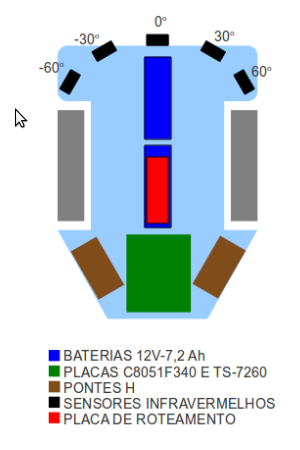
\includegraphics[width=0.4\textwidth]{./figuras/disposicao-robo.png}
\caption[Disposição dos itens no robô]{Disposição dos itens no robô}
\fonte{\cite{bellator_2012}}
\label{fig:disposicao_bellator_2012}
\end{figure}

\subsubsection{Odometria}

Para a obtenção da direção e sentido do movimento do robô, assim como aceleração, velocidade e posição, pode-se optar por diversos tipos de tecnologias ou pela associação delas. Abaixo descrevemos as principais delas.

\begin{itemize}
  \item \textbf{Encoder:} Ligado ao eixo da roda do robô, conta a quantidade de voltas dadas pela roda. Permite assim calcular a distancia percorrida pelo robô. Caso sejam conectados dois encoders, um em cada roda, podemos obter também a direção do movimento pela diferença entre a contagem de voltas de cada roda.
  \item \textbf{GPS:} Utiliza sinais de satélites para obter as coordenadas geográficas do robô. A direção e o sentido podem ser obtidos pela comparação das leituras com as anteriores.
  \item 	\textbf{Acelerômetro:} pode utilizar a tecnologia chamada \textbf{MEMS} para medir a aceleração sofrida pelo componente.
  \item 	\textbf{Giroscópio:} pode utilizar a tecnologia chamada \textbf{MEMS} para medir a aceleração angular sofrida pelo componente.
  \item 	\textbf{Bussola:} Utiliza os campos magnéticos da terra para obter a direção com relação aos polos magnéticos da terra.
\end{itemize}

A seguir, na tabela \ref{tab:alternativas_tecnologias_odometria}, comparamos as tecnologias apresentadas anteriormente. 

\begin{table}[h]
  \caption{Comparação entre tecnologias para odometria.}
  \centering
  \begin{tabular}{p{3cm}|p{2.2cm}p{1.7cm}p{2.2cm}p{2.2cm}p{2.2cm}}
    \toprule
    \textbf{Característica} & \textbf{Encoder} & \textbf{GPS} & \textbf{Acelerômetro} & \textbf{Giroscópio} & \textbf{Bussola} \\
    \hline
    Sujeito a influencias externas & Deslizamentos & Não & Não & Não & Campo magnético dos motores \\
    \hline
    Ambiente de operação & Interno / Externo & Externo & Interno / Externo & Interno / Externo & Interno / Externo \\
    \hline
    Posicionamento & Relativo & Absoluto & Relativo & Relativo & Relativo \\
    \bottomrule
  \end{tabular}
  \label{tab:alternativas_tecnologias_odometria}
\end{table}

Com base no comparativo da tabela \ref{tab:alternativas_tecnologias_odometria} optamos por utilizar um acelerômetro em conjunto com um giroscópio para obter os dados para odometria. Encoders estão sujeitos a erros causados por deslizamento nas rodas, GPS apenas funciona em ambientes externos e a bussola pode ser influenciada pelo campo magnético dos motores. Como o robô já apresenta encoders instalado, utilizaremos também os dois encoders, possibilitando assim aumentar a precisão e confiabilidade dos dados de odometrias.
Justificada nossa escolha por acelerômetros e giroscópios, na tabela \ref{tab:alternativas_componentes_odometria} fazemos um comparativo entre as opções de menor custo disponíveis no mercado. Listamos na tabela apenas as alternativas que possuem placas de desenvolvimento pois acelerômetros e giroscópios são geralmente são vendidos em encapsulamento LGA, os quais são de difícil soldagem.

\begin{table}[h]
  \caption{Comparação entre acelerômetros/giroscópios para odometria.}
  \centering
  \begin{tabular}{p{2.4cm}|p{3cm}p{0.8cm}p{1.4cm}p{1.8cm}p{1.7cm}p{1.3cm}}
    \toprule
    \textbf{Modelo} & \textbf{Fabricante} & \textbf{Acel.} & \textbf{Giro.} & \textbf{Faixa} & \textbf{Interface} & \textbf{Preço} \\
    \hline
    STEVAL-MKI009V1	& STMicroeletronics & 3x	& - & $ \pm 2g / \pm6g $ & I2c / SPI & \$23.94 \\
    \hline
	ATAVRSBIN1 & Atmel & 1x & - & - & I2c & \$26.25 \\
	\hline
	KIT3803 MMA7660FC & Freescale & 3x & - & $ \pm 1.5g $ & I2C & 	\$35.0 \\
	\hline
	ATAVRSBIN1 & Atmel & - & 1x & & I2C & \$26.25 \\
	\hline
	MPU-6050	 & IvenSense & 3x & 3x & $ \pm 2g / \pm 4g $ $ \pm 250 ^{o}/seg /$ $ \pm 500 ^{o}/seg $ & I2C & \$8.78 \\
    \hline
	MKI086V1	 & STMicroeletronics & 1x & $ \pm 30^{o}/seg $ & Analog & & \$31.50 \\
	\hline
	STEVAL-MKI094V1 & STMicroeletronics & - & 3x & $ \pm 400^{o}/seg $ & Analog & \$31.50 \\
	\hline
	ATAVRSBIN1 & Atmel & 1x & 1x & & I2C & \$26.25 \\
	\hline
	DM240316	 & Zena & 3x & 3x & 	& RF & \$99.99 \\
    \bottomrule
  \end{tabular}
  \label{tab:alternativas_componentes_odometria}
\end{table}

\textbf{MPU-6050}

Com base na tabela \ref{tab:alternativas_componentes_odometria} escolhemos o modelo MPU-6050 da IvenSense principalmente devido ao seu baixo custo: \$8.78. Este modelo possui um acelerômetro de 3 eixos, um giroscópio e 3 eixos e entradas para uma bussola externa integrados em um único chip \cite{mpu6050}. A faixa de operação para o acelerômetro é de $ \pm 2g ou \pm 4g $ e para o giroscópio é de $ \pm 250 ^{o}/seg $ ou $ \pm 500 ^{o}/seg $. A sensibilidade do acelerômetro é de $ 16384 LSB/g $ e $ 8192 LSB/g $. A sensibilidade do giroscópio é de $ 131 LSB/ ^{o} / seg $ e $ 65.5 LSB/ ^{o} / seg $. A interface de comunicação do módulo suporta o protocolo I2C. O módulo contendo o chip MPU-6050 e alguns componentes necessários para seu funcionamento pode ser visto na figura \ref{fig:mpu6050}.

\begin{figure}[H]
\centering
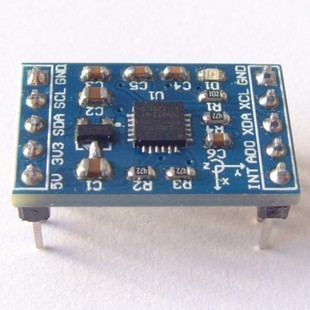
\includegraphics[width=0.4\textwidth]{./figuras/mpu6050.JPG}
\caption[Placa de desenvolvimento contendo o chip MPU-6050]{Placa de desenvolvimento contendo o chip MPU-6050}
\fonte{\cite{mpu6050}}
\label{fig:mpu6050}
\end{figure}

\textbf{Encoder Optico HEDS-9700}

Como já foi dito, utilizaremos também os encoders já existentes no robô. O robô está equipado com dois encoders HEDS-9700.
Esses encoders geram em sua saída uma onda quadrada à medida em que o encoder é rotacionado, sendo 1800 pulsos gerados em uma rotação \cite{heds9700}. A forma de onda da saída do encoder pode ser vista na figura \ref{fig:heds9700}. Podemos ver na figura que o encoder possui duas saidas, A e B com defasamento $\phi$ entre elas. Com as duas saídas podemos determinar o sentido de rotação. Porém na implementação existente esse recurso não é utilizado.

\begin{figure}[H]
\centering
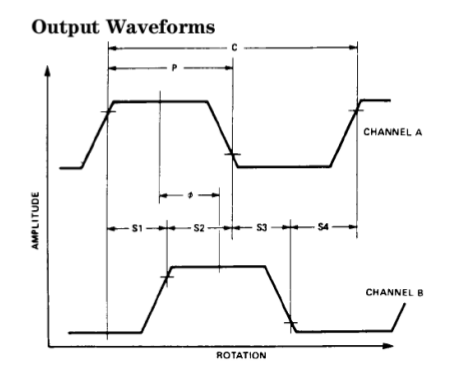
\includegraphics[width=0.6\textwidth]{./figuras/heds9700.png}
\caption[Forma de onda de saída do encoder]{Forma de onda de saída do encoder}
\fonte{\cite{heds9700}}
\label{fig:heds9700}
\end{figure}

\subsubsection{Detecção de obstáculos}

\textbf{Sensor de proximidade Infra Vermelho IR 2Y0A02F98}

A detecção de obstáculos, que é um requisito deste robô, será atendido pelos sensores de Infra vermelho já existentes no robô. Logo serão utilizados sensores IR 2Y0A02F98 \cite{ir_sensor}. Este modelo é pouco influenciado pelas cores dos objetos detectados devido ao método de medição baseado em triangulação. Na figura \ref{fig:ir_sensor_response} podemos ver isso. A linha tracejada é a resposta para reflexão em um papel cinza e a linha contínua é a resposta para reflexão em um papel branco.

\begin{figure}[H]
\centering
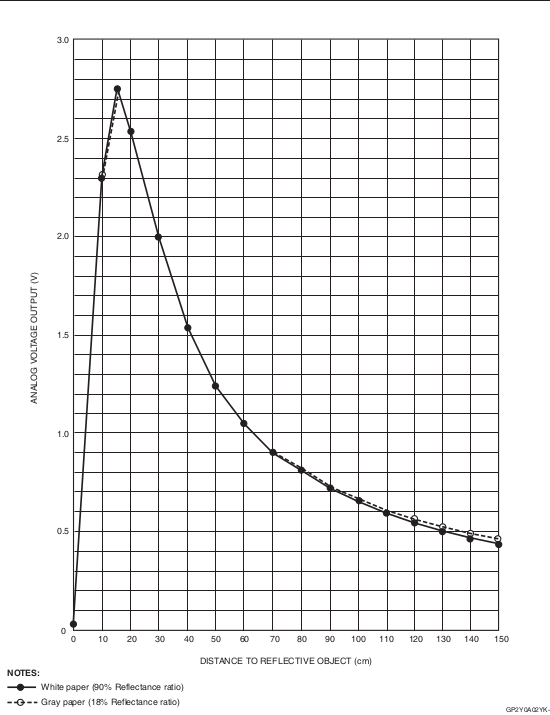
\includegraphics[width=1\textwidth]{./figuras/ir-sensor-response.png}
\caption[Curva de resposta do encoder]{Curva de resposta do encoder}
\fonte{\cite{ir_sensor}}
\label{fig:ir_sensor_response}
\end{figure}

\subsubsection{Microcontrolador}

A interface entre os sensores, atuadores e a placa TS-7260 já existente no robô \cite{bellator_2012} será feita por um sistema micro controlado. Uma vez escolhidos os sensores, o sistema micro controlado deve possuir as interfaces adequadas para comunicação com os sensores e também para comunicação com o hardware já existente no robô, como o sistema de acionamento dos motores e interface com a placa TS-7260. Desta forma, na tabela \ref{tab:requisitos_microcontrolador} listamos os requisitos para escolha do microcontrolador. Na tabela \ref{tab:requisitos_desejaveis_microcontrolador} listamos os requisitos que não são obrigatórios, porém desejáveis para o microcontrolador.

\begin{table}[h]
  \caption{Requisitos para escolha do microcontrolador.}
  \centering
  \begin{tabular}{p{7cm}|p{8cm}}
    \toprule
    \textbf{Requisito} & \textbf{Justificativa} \\
    \hline
    Interface I2C & Comunicação com acelerômetro e giroscópio \\
    \hline
    Geração de PWM em 4 canais & Acionamento dos motores pelas pontes H \\
    \hline
    Interface Serial	 & Comunicação com a placa TS-7260 \\
    \hline
    Interrupções em 2 canais	 & Leitura do valor dos encoders \\
    \hline
    Conversor AD em 5 canais	 & Leitura dos sensores de IR \\
    \bottomrule
  \end{tabular}
  \label{tab:requisitos_microcontrolador}
\end{table}

\begin{table}[h]
  \caption{Requisitos desejáveis para escolha do microcontrolador.}
  \centering
  \begin{tabular}{p{7cm}|p{8cm}}
    \toprule
    \textbf{Requisito desejável} & \textbf{Justificativa} \\
    \hline
    Desenvolvimento em plataforma livre	 & Diminui o custo de softwares para desenvolvimento \\
    \hline
    32 bits & Facilita manipulações numéricas na programação, diminuindo esforço e custo para programação \\
    \hline
    2 Interfaces seriais ou JTAG & Utilização para debug ou logs \\
    \hline
    Solução integrada & Redução do tamanho da placa e quantidade de componentes, diminuindo assim o custo e melhorando a organização e disposição dos componentes \\
    \bottomrule
  \end{tabular}
  \label{tab:requisitos_desejaveis_microcontrolador}
\end{table}

Na tabela \ref{tab:alternativas_microcontrolador} listamos diversas opções de microcontroladores que foram pesquisados para o projeto. Todas as opções atendem aos requisitos da tabela \ref{tab:requisitos_microcontrolador}, e são 32 bits.

\begin{table}[h]
\caption{Comparativo entre microcontroladores.}
\fonte{Dados obtidos de \cite{digikey}}
\centering
\begin{tabular}{l|rrrrrr}
\toprule
\textbf{uC} & \textbf{STM32F103C6T7A} & \textbf{PIC32MX320F128H} & \textbf{LPC2103} \\ \hline
Fabricante & STMicroelectronics & Microchip Technology & NXP Semiconductors \\ \hline
Arquitetura & ARM® Cortex™-M3 & MIPS32® M4K™ & ARM7 \\ \hline
Core & 32bits & 32-Bit & 16/32-Bit \\ \hline
Velocidade & 72MHz & 80MHz & 70MHz \\ \hline
MIPS & 90 & 124.8 & 63 \\ \hline
I2C & 1 & 2 & 2 \\ \hline
PWM & 12 & 5 & 14 \\ \hline
UART & 2 & 2 & 2 \\ \hline
Einterrupt & 16 & 5 & 13 \\ \hline
FLASH & 32k & 128k & 32k \\ \hline
RAM & 10k & 16k & 8k \\ \hline
Adc & 10x12b & 16x10b & 8x10b \\ \hline
JTAG & sim & sim & sim \\ \hline
Custo & \$6.27 & \$6.26 & \$6.16 \\
\toprule
\textbf{uC} & \textbf{MCF52210CAE66} & \textbf{AT32UC3C264C} & \textbf{SIM3C146} \\ \hline
Fabricante & Freescale Semiconductor & Atmel & Silicon Laboratories Inc \\ \hline
Arquitetura & Coldfire V2 & AVR & ARM® Cortex™-M3 \\ \hline
Core & 32-Bit & 32-Bit & 32-Bit \\ \hline
Velocidade & 66MHz & 66MHz & 80MHz \\ \hline
MIPS & 75.9 & 98.34 & 100 \\ \hline
I2C & 2 & 3 & 2 \\ \hline
PWM & 4 & 8 & 8 \\ \hline
UART & 3 & 1 & 2 \\ \hline
Einterrupt & 7 & 7 & 16 \\ \hline
FLASH & 64k & 64k & 64k \\ \hline
RAM & 16k & 16k & 16k \\ \hline
Adc & 8x12b & 11x12b & 28x12b \\ \hline
JTAG & sim & sim & SIM3C146-B-GQ \\ \hline
Custo & \$7.1 & \$9.14 & \$6.1 \\ \bottomrule
\end{tabular}
\label{tab:alternativas_microcontrolador}
\end{table}

Dentre as opções listadas na tabela \ref{tab:alternativas_microcontrolador} escolhemos a opção \textbf{LPC2103}. Esta escolha foi feita baseada principalmente no custo do microcontrolador. Porém ao compará-lo com o \textbf{SIM3C146} vemos que esta última opção possui desempenho melhor com custo menor. Nossa escolha pelo \textbf{LPC2103} e não pelo \textbf{SIM3C146} justifica-se pela melhor documentação e disponibilidade de recursos para o \textbf{LPC2103}. A documentação fornecida pelo fabricante do microcontrolador \textbf{LPC2103} é mais completa, e por já estar a mais tempo no mercado a quantidade de informações e recursos disponíveis na internet é maior.

\textbf{LCP2103}

O \textbf{LCP2103} é um microcontrolador baseado na arquitetura ARM7TDMI-S da NXP \cite{lpc2103}. Este microcontrolador pode operar em até $ 70MHz $ executando a $ 63MIPS $. O Microcontrolador possui 2 interfaces I2C, 2 interfaces seriais, até 14 saídas de PWM, até 13 canais de interrupções externas, 8 canais de conversão para um conversor analógico digital de 10 bits, 32kbytes de memória FLASH para código e 8kbytes de memória RAM. Ele também suporta \textit{debug} via JTag por meio de um \textit{debugger} JTag externo. O custo desse microcontrolador é de \$6.16 \cite{digikey}.

O microcontrolador escolhido também pode ser programado utilizando o protocolo ISP por meio de ferramentas livres como o lpc21isp \cite{lpc21isp}. Para geração do código hexadecimal utilizado pelo lpc21isp basta compilar o código em C utilizando o GCC \cite{gcc}.
Portanto o \textbf{LCP2103} além de atender aos requisitos propostos anteriormente também atende aos requisitos desejáveis que foram propostos na tabela \ref{tab:requisitos_desejaveis_microcontrolador}.
